\documentclass[12pt,a4paper]{article}
\usepackage[utf8]{inputenc}
\usepackage[T1]{fontenc}
\usepackage{times}
\usepackage{geometry}
\geometry{top=3cm, bottom=3cm, left=3cm, right=3cm} 
\usepackage{amsmath, amssymb, amsfonts}
\usepackage{graphicx}
\usepackage{booktabs}
\usepackage{array}
\usepackage{titlesec}
\usepackage{lipsum}
\usepackage{fancyhdr}
\usepackage{listings}
\usepackage{setspace}
\usepackage{xcolor}
\usepackage{tikz}

% --- KONFIGURASI WARNA ---
\definecolor{itbblue}{RGB}{0, 94, 184}

% --- KONFIGURASI JUDUL BAB (HITAM & BOLD) ---
\titleformat{\section}
  {\normalfont\Large\bfseries}{\thesection}{1em}{}[{\titlerule[1pt]}]
\titleformat{\subsection}
  {\normalfont\large\bfseries}{\thesubsection}{1em}{}

% --- Konfigurasi Bahasa ---
\renewcommand{\figurename}{Gambar}
\renewcommand{\tablename}{Tabel}

% --- KONFIGURASI CODE LISTING ---
\lstset{
    basicstyle=\ttfamily\small,
    breaklines=true,
    numbers=left,
    numbersep=5pt,
    frame=single,
    tabsize=2
}

\begin{document}

% --- HALAMAN COVER (MENGIKUTI CONTOH GAMBAR) ---
\begin{titlepage}
    \centering
    \setstretch{1.5} % Spasi agak lebar untuk cover
    
    {\large\bfseries LAPORAN TUGAS \#2}\\[0.5cm]
    
    {\Large\bfseries DISTRIBUSI TEMPERATUR KONDISI TUNAK BENDA 2D DENGAN METODE BEDA-HINGGA (MBH)}\\[2cm]
    
    % --- BAGIAN LOGO (MASUKKAN GAMBAR DI SINI) ---
    
\includegraphics[width=5cm]{figures/logo_itb.jpg} \\[2cm]
    
    {\normalsize Laporan ini Disusun Untuk Memenuhi Tugas Mata Kuliah\\
    IK5025 Pengukuran, Pemodelan, dan Simulasi Komputasional}\\[1cm]
    
    {\normalsize\bfseries Disusun Oleh :}\\[0.5cm]
    
    \begin{center}
    \setstretch{1.2}
    \begin{tabular}{lcl}
        Nama & : & Izma Alhazmi Herdian \\
        NIM  & : & 23825301 \\
    \end{tabular}
    \end{center}
    
    \vfill
    
    % --- FOOTER KAMPUS ---
    {\normalsize\bfseries PROGRAM STUDI MAGISTER INSTRUMENTASI DAN KONTROL\\
    FAKULTAS TEKNOLOGI INDUSTRI\\
    INSTITUT TEKNOLOGI BANDUNG\\
    2026}

\end{titlepage}

\newpage
% --- PENGATURAN HALAMAN ISI ---
\pagestyle{fancy}
\fancyhf{}
\lhead{\small IK5025 Simulasi Komputasional}
\rhead{\small Tugas \#2}
\rfoot{\thepage}
\setstretch{1.15} 

% --- SECTION 1: DESKRIPSI SOAL ---
\section{Deskripsi Soal dan Geometri Sistem}
Tugas ini bertujuan untuk memodelkan dan menghitung distribusi temperatur pada kondisi tunak (\textit{steady-state}) untuk sebuah pelat dua dimensi (2D). Perhitungan dilakukan menggunakan \textbf{Metode Beda-Hingga (MBH)} berdasarkan prinsip dasar konduksi termal yang diuraikan oleh Incropera dkk. \cite{incropera_principles_2013}. Rincian geometri, kondisi batas, serta parameter simulasi yang digunakan dijelaskan sebagai berikut:

\subsection{Geometri dan Material Benda}
\begin{itemize}
    \item Pelat 2D memiliki dimensi terluar sebesar $1\text{ m} \times 1\text{ m}$.
    \item Terdapat area kosong tepat di tengah pelat dengan dimensi panjang $a = 0.25\text{ m}$ dan lebar $b = 0.25\text{ m}$. Area ini bertindak sebagai \textbf{isolator panas (\textit{heat insulator})}, sehingga nilai pembangkitan fluks kalor pada batas tersebut diasumsikan bernilai nol.
    \item Material pelat merupakan golongan logam. Untuk keperluan analisis komparatif, pemodelan akan dilakukan menggunakan \textbf{dua variasi jenis logam} yang memiliki nilai konduktivitas termal berbeda.
\end{itemize}

\subsection{Kondisi Batas (\textit{Boundary Conditions})}
Sistem ini diekspos pada kondisi batas suhu tetap (\textit{Dirichlet Boundary Condition}) pada keempat sisi terluar pelat, dengan rincian distribusi temperatur sebagai berikut:
\begin{itemize}
    \item \textbf{Sisi Kiri:} $T_{\text{kiri}} = 100^\circ\text{C}$
    \item \textbf{Sisi Kanan:} $T_{\text{kanan}} = 20^\circ\text{C}$
    \item \textbf{Sisi Atas:} $T_{\text{atas}} = 20^\circ\text{C}$
    \item \textbf{Sisi Bawah:} $T_{\text{bawah}} = 50^\circ\text{C}$
\end{itemize}
Sementara itu, pada batas area tengah berukuran $0.25\text{ m} \times 0.25\text{ m}$, berlaku kondisi batas \textit{Neumann} (isolator termal) di mana gradien temperatur terhadap arah normal permukaan adalah nol ($\frac{\partial T}{\partial n} = 0$). Skema geometri dan kondisi batas sistem secara detail dapat dilihat pada Gambar 1.

\begin{center}
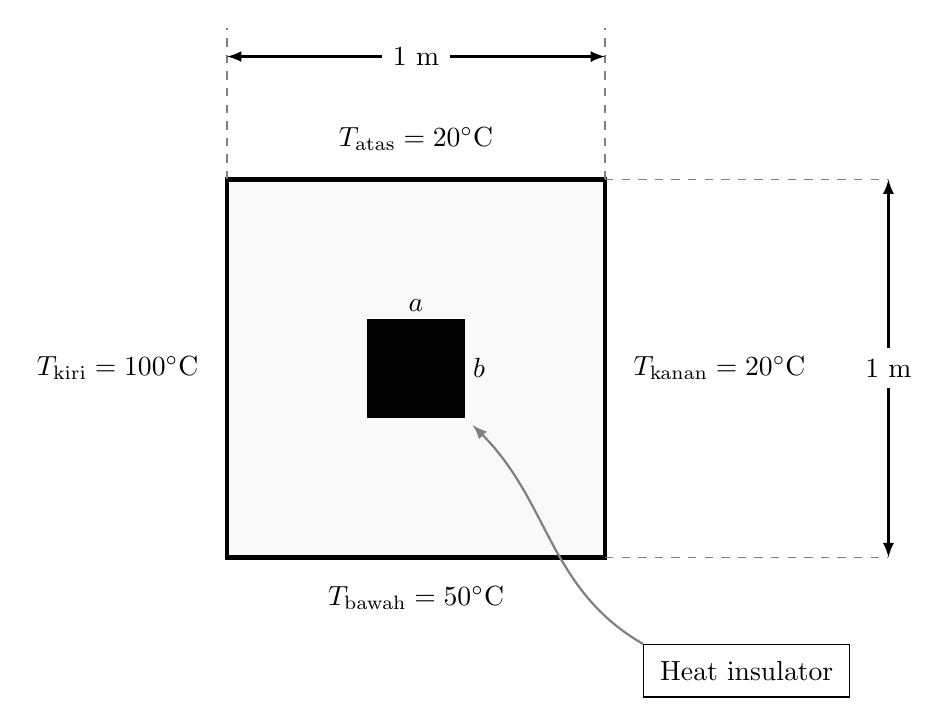
\begin{tikzpicture}[scale=1.2, >=latex]
    % 1. Batas Luar Pelat
    \draw[ultra thick, fill=gray!5] (0,0) rectangle (4,4);
    
    % 2. Insulator di Tengah
    \draw[ultra thick, fill=black] (1.5,1.5) rectangle (2.5,2.5);
    
    % 3. Label Dimensi Insulator (a dan b)
    \node[above] at (2, 2.5) {$a$};
    \node[right] at (2.5, 2) {$b$};
    
    % 4. Kondisi Batas Suhu (Dirichlet) - Menggunakan subscript
    \node[above] at (2, 4.2) {$T_{\text{atas}} = 20^\circ\text{C}$};
    \node[below] at (2, -0.2) {$T_{\text{bawah}} = 50^\circ\text{C}$};
    \node[left]  at (-0.2, 2) {$T_{\text{kiri}} = 100^\circ\text{C}$};
    \node[right] at (4.2, 2) {$T_{\text{kanan}} = 20^\circ\text{C}$};
    
    % 5. Garis Bantu dan Dimensi Atas (1 m)
    % Digeser lebih ke atas (y = 5.6) agar tidak menabrak teks suhu
    \draw[gray, thin, dashed] (0,4) -- (0,5.6);
    \draw[gray, thin, dashed] (4,4) -- (4,5.6);
    \draw[<->, thick] (0,5.3) -- (4,5.3) node[midway, fill=white, inner sep=4pt] {$1\text{ m}$};
    
    % 6. Garis Bantu dan Dimensi Kanan (1 m)
    % Digeser lebih ke kanan (x = 6.6) agar tidak menabrak teks suhu
    \draw[gray, thin, dashed] (4,0) -- (7,0);
    \draw[gray, thin, dashed] (4,4) -- (7,4);
    \draw[<->, thick] (7,0) -- (7,4) node[midway, fill=white, inner sep=4pt] {$1\text{ m}$};
    
    % 7. Keterangan "Heat insulator"
    % Diposisikan agar panahnya melengkung rapi ke kotak hitam
    \node[draw, fill=white, inner sep=6pt] (insulator) at (5.5, -1.2) {Heat insulator};
    \draw[->, thick, gray, out=150, in=-45] (insulator.north west) to (2.6, 1.4);
\end{tikzpicture}
\\ \vspace{0.3cm}
\small\textit{Gambar 1: Skema Geometri, Kondisi Batas, dan Dimensi Pelat 2D}
\end{center}

\subsection{Skenario Simulasi dan Luaran}
Dalam penyelesaian komputasionalnya, beberapa skenario dan luaran yang diwajibkan adalah:
\begin{itemize}
    \item \textbf{Variasi Kisi (\textit{Grid}):} Analisis pemodelan dilakukan dengan memvariasikan ukuran langkah spasial atau jarak antar \textit{node} ($\Delta x$ dan $\Delta y$), dengan ketentuan bahwa grid yang digunakan beraturan, yaitu $\Delta x = \Delta y$.
    \item \textbf{Luaran Data:} Menghasilkan dan menampilkan data distribusi temperatur untuk setiap titik \textit{node} komputasi dalam sistem matriks.
    \item \textbf{Representasi Visual:} Memplot hasil distribusi temperatur tersebut ke dalam representasi gambar 2D (\textit{contour plot}) agar profil perpindahan dan gradien suhu dapat diamati secara intuitif.
\end{itemize}

% --- SECTION 2: ASUMSI MODEL ---
\section{Asumsi Model}
Dalam melakukan pemodelan dan simulasi komputasional distribusi temperatur ini, diterapkan beberapa asumsi dasar fisis dan matematis sebagai berikut:
\begin{enumerate}
    \item \textbf{Kondisi Tunak (\textit{Steady-State}):} Sistem diasumsikan telah mencapai kesetimbangan termal terhadap waktu, sehingga tidak ada akumulasi atau penipisan energi di dalam pelat. Laju perubahan temperatur terhadap waktu bernilai nol ($\frac{\partial T}{\partial t} = 0$).
    \item \textbf{Perpindahan Panas Dua Dimensi (2D):} Dimensi ketebalan pelat (sumbu-$z$) diabaikan atau dianggap cukup tipis sehingga gradien temperatur pada arah tersebut sangat kecil. Perpindahan panas dominan hanya terjadi pada bidang $x$ dan $y$.
    \item \textbf{Material Homogen dan Isotropik:} Properti termal material logam, khususnya konduktivitas termal ($k$), diasumsikan konstan di seluruh bagian pelat, memiliki nilai yang sama ke segala arah, dan tidak bergantung pada perubahan temperatur.
    \item \textbf{Tanpa Pembangkitan Kalor Internal:} Kecuali pada area insulasi yang memang didefinisikan memiliki fluks nol, material pelat logam itu sendiri diasumsikan tidak memiliki sumber pembangkitan panas internal ($\dot{q} = 0$). Hal ini menyederhanakan persamaan Poisson menjadi persamaan Laplace ($\nabla^2 T = 0$) untuk \textit{interior node}.
    \item \textbf{Insulasi Termal Ideal:} Area berukuran $0.25\text{ m} \times 0.25\text{ m}$ di tengah pelat diasumsikan sebagai isolator sempurna. Tidak ada fluks kalor yang menembus batas area tersebut, sehingga kondisi batas Neumann ($\frac{\partial T}{\partial n} = 0$) berlaku mutlak pada batas antarmuka logam-isolator.
\end{enumerate}

% --- SECTION 3: METODOLOGI DAN DISKRITISASI ---
\section{Metodologi dan Diskritisasi Beda-Hingga}
Pemodelan distribusi temperatur pada tugas ini diselesaikan menggunakan Metode Beda-Hingga (MBH). Untuk memperoleh formulasi numerik yang akurat, persamaan diturunkan dari persamaan pembangun (\textit{governing equation}) fundamental, kemudian dievaluasi berdasarkan lokalisasi titik pada area komputasi.

\subsection{Penurunan Persamaan Pembangun (\textit{Governing Equation})}
Berdasarkan Hukum Kekekalan Energi dan Hukum Fourier, persamaan umum difusi kalor (\textit{heat diffusion equation}) dalam koordinat Kartesian tiga dimensi dinyatakan sebagai \cite{incropera_principles_2013}:
\begin{equation} \label{eq:heat_diffusion}
    \frac{\partial}{\partial x} \left( k \frac{\partial T}{\partial x} \right) + \frac{\partial}{\partial y} \left( k \frac{\partial T}{\partial y} \right) + \frac{\partial}{\partial z} \left( k \frac{\partial T}{\partial z} \right) + \dot{q} = \rho c_p \frac{\partial T}{\partial t}
\end{equation}

Sistem pada tugas ini dievaluasi pada kondisi tunak (\textit{steady-state}) sehingga laju perubahan energi terhadap waktu bernilai nol ($\frac{\partial T}{\partial t} = 0$). Selain itu, perpindahan panas ditinjau dominan dalam dua dimensi ($x$ dan $y$), dan nilai konduktivitas termal material ($k$) diasumsikan konstan di seluruh domain logam. Dengan menerapkan kondisi-kondisi tersebut pada Persamaan (\ref{eq:heat_diffusion}), diperoleh Persamaan Poisson 2D:
\begin{equation} \label{eq:poisson}
    \frac{\partial^2 T}{\partial x^2} + \frac{\partial^2 T}{\partial y^2} + \frac{\dot{q}}{k} = 0
\end{equation}

Lebih lanjut, karena material pelat pada kasus ini diasumsikan tidak memiliki sumber pembangkitan kalor internal ($\dot{q} = 0$), Persamaan Poisson (\ref{eq:poisson}) tereduksi menjadi bentuk akhirnya yaitu Persamaan Laplace 2D:
\begin{equation} \label{eq:laplace}
    \frac{\partial^2 T}{\partial x^2} + \frac{\partial^2 T}{\partial y^2} = 0
\end{equation}

\subsection{Analisis Skenario Node dan Diskritisasi}
Proses diskritisasi komputasional dilakukan dengan memetakan domain kontinu pelat 2D berukuran $1\text{ m} \times 1\text{ m}$ ke dalam sebuah jaringan kisi spasial (\textit{spatial grid}) diskrit. Domain tersebut dibagi menjadi matriks titik-titik pias (\textit{nodes}) dengan jarak antar titik sebesar $\Delta x$ pada arah horizontal dan $\Delta y$ pada arah vertikal. Mengingat analisis ini menggunakan resolusi kisi seragam ($\Delta x = \Delta y$), setiap koordinat fisik $(x,y)$ direpresentasikan dengan presisi oleh indeks matriks $(m,n)$.

Keberadaan isolator panas berukuran $0.25\text{ m} \times 0.25\text{ m}$ tepat di pusat pelat menyebabkan domain komputasi tidak lagi berupa bidang persegi homogen, melainkan memiliki "lubang" fisis (batas adiabatik internal). Diskritisasi keseluruhan pelat beserta letak elemen-elemen spesifiknya divisualisasikan pada Gambar 2.

\begin{figure}[h!]
\centering
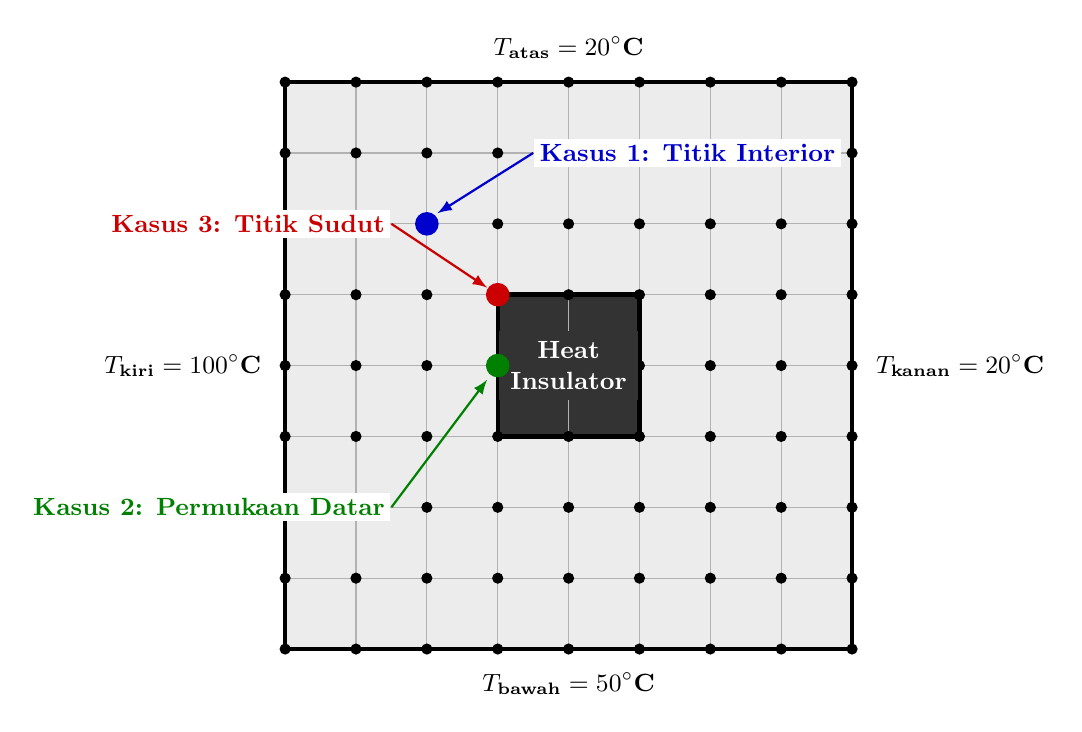
\begin{tikzpicture}[scale=0.9, >=latex]
    % --- LAYER 1: LATAR LOGAM DAN ISOLATOR ---
    \fill[gray!15] (0,0) rectangle (8,8);
    \fill[black!80] (3,3) rectangle (5,5);

    % --- LAYER 2: GARIS GRID ---
    \draw[step=1.0, gray!60, thin] (0,0) grid (8,8);

    % --- LAYER 3: BATAS TEGAS ---
    \draw[ultra thick, black] (3,3) rectangle (5,5); % Batas Isolator
    \draw[ultra thick, black] (0,0) rectangle (8,8); % Batas Luar Pelat

    % --- LAYER 4: TITIK NODE KESELURUHAN ---
    % Loop untuk menggambar semua titik persimpangan grid
    \foreach \x in {0,...,8} {
        \foreach \y in {0,...,8} {
            \filldraw[black] (\x,\y) circle (2pt);
        }
    }

    % --- LAYER 5: TEKS ISOLATOR (Menimpa titik di tengah) ---
    \node[white, font=\small\bfseries, align=center, fill=black!80, inner sep=4pt] at (4,4) {Heat\\Insulator};

    % --- LAYER 6: KONDISI BATAS (Sisi Luar) ---
    \node[above, font=\small\bfseries] at (4,8.2) {$T_{\text{atas}} = 20^\circ\text{C}$};
    \node[below, font=\small\bfseries] at (4,-0.2) {$T_{\text{bawah}} = 50^\circ\text{C}$};
    \node[left, font=\small\bfseries]  at (-0.2,4) {$T_{\text{kiri}} = 100^\circ\text{C}$};
    \node[right, font=\small\bfseries] at (8.2,4) {$T_{\text{kanan}} = 20^\circ\text{C}$};

    % --- LAYER 7: HIGHLIGHT KASUS 1, 2, dan 3 ---
    % Warna khusus untuk penanda
    \colorlet{colorK1}{blue!80!black}
    \colorlet{colorK2}{green!50!black}
    \colorlet{colorK3}{red!80!black}

    % Kasus 1: Interior Node (Titik biru, misalnya di koordinat m=2, n=6)
    \filldraw[colorK1] (2,6) circle (4.5pt);
    \draw[<-, thick, colorK1] (2.15, 6.15) -- (3.5, 7) node[right, font=\small\bfseries, fill=white, inner sep=2pt] {Kasus 1: Titik Interior};

    % Kasus 2: Permukaan Datar Isolator (Titik hijau, di tepi kiri isolator m=3, n=4)
    \filldraw[colorK2] (3,4) circle (4.5pt);
    \draw[<-, thick, colorK2] (2.85, 3.8) -- (1.5, 2) node[left, font=\small\bfseries, fill=white, inner sep=2pt] {Kasus 2: Permukaan Datar};

    % Kasus 3: Sudut Dalam Isolator (Titik merah, di pojok kiri-atas m=3, n=5)
    \filldraw[colorK3] (3,5) circle (4.5pt);
    \draw[<-, thick, colorK3] (2.85, 5.10) -- (1.5, 6) node[left, font=\small\bfseries, fill=white, inner sep=2pt] {Kasus 3: Titik Sudut};

\end{tikzpicture}
\caption{Pemetaan kisi spasial (\textit{grid}) pada domain komputasi pelat logam. Keberadaan \textit{heat insulator} di bagian tengah melahirkan tiga klasifikasi \textit{node} yang memerlukan formulasi diskritisasi berbeda.}
\label{fig:overall_grid}
\end{figure}

Berdasarkan pemetaan spasial pada Gambar~\ref{fig:overall_grid}, secara fisis terdapat tiga klasifikasi elemen fisis yang dievaluasi. Formulasi turunan untuk masing-masing titik diselesaikan menggunakan \textbf{Metode Kesetimbangan Energi} ($\sum q_{\text{in}} = 0$) pada \textit{control volume} masing-masing \textit{node} sebagai berikut:

\subsubsection*{Kasus 1: Titik Interior (\textit{Interior Nodes})}
Titik interior berada sepenuhnya di dalam domain logam yang homogen (Gambar~\ref{fig:kasus_1}). Karena fungsi temperatur diasumsikan kontinu di area ini, Persamaan Laplace (\ref{eq:laplace}) dapat langsung didiskritisasi menggunakan pendekatan beda pusat (\textit{central difference}) dari Deret Taylor orde dua:
\begin{equation} \label{eq:taylor_x}
    \frac{\partial^2 T}{\partial x^2} \approx \frac{T_{m+1,n} - 2T_{m,n} + T_{m-1,n}}{(\Delta x)^2}
\end{equation}
\begin{equation} \label{eq:taylor_y}
    \frac{\partial^2 T}{\partial y^2} \approx \frac{T_{m,n+1} - 2T_{m,n} + T_{m,n-1}}{(\Delta y)^2}
\end{equation}

\begin{figure}[h!]
\centering
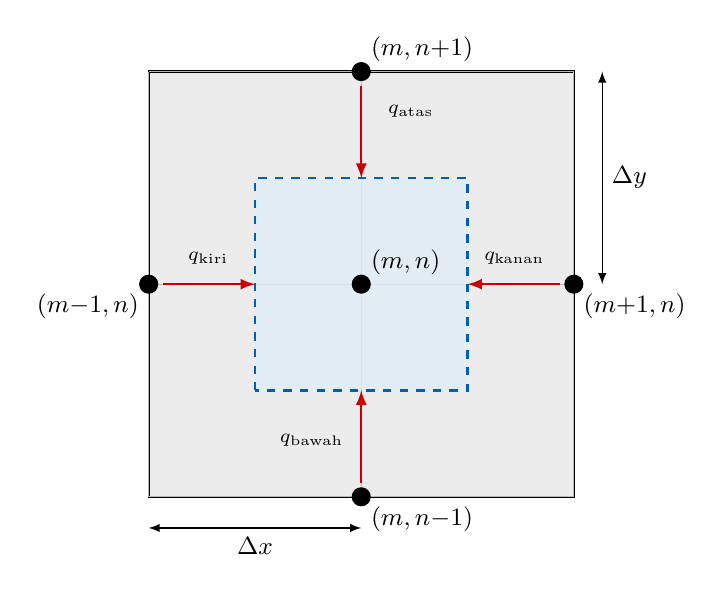
\begin{tikzpicture}[scale=1.8, >=latex]
    \colorlet{metal}{gray!15}
    \fill[metal] (-1.5,-1.5) rectangle (1.5, 1.5);
    \draw[black, thick] (-1.5,-1.5) rectangle (1.5,1.5);
    \foreach \x in {-1.5, 0, 1.5} \draw[gray!55, thin] (\x,-1.5) -- (\x,1.5);
    \foreach \y in {-1.5, 0, 1.5} \draw[gray!55, thin] (-1.5,\y) -- (1.5,\y);
    \draw[dashed, thick, itbblue, fill=itbblue!12, fill opacity=0.8] (-0.75,-0.75) rectangle (0.75,0.75);
    
    \draw[<->, thin, black] (-1.5,-1.72) -- (0,-1.72) node[midway, below, font=\small] {$\Delta x$};
    \draw[<->, thin, black] (1.7,0) -- (1.7,1.5) node[midway, right, font=\small] {$\Delta y$};
    
    \draw[->, thick, red!80!black] (-1.40, 0.0) -- (-0.75, 0.0);
    \node[font=\scriptsize, black] at (-1.08, 0.18) {$q_\text{kiri}$};
    \draw[->, thick, red!80!black] (0.0, 1.40) -- (0.0, 0.75);
    \node[font=\scriptsize, black] at (0.35, 1.22) {$q_\text{atas}$};
    \draw[->, thick, red!80!black] (1.40, 0.0) -- (0.75, 0.0);
    \node[font=\scriptsize, black] at (1.08, 0.18) {$q_\text{kanan}$};
    \draw[->, thick, red!80!black] (0.0, -1.40) -- (0.0, -0.75);
    \node[font=\scriptsize, black] at (-0.35, -1.10) {$q_\text{bawah}$};
    
    \filldraw[black] ( 0.0,  0.0) circle (1.8pt) node[above right, font=\small] {$(m,n)$};
    \filldraw[black] (-1.5,  0.0) circle (1.8pt) node[below left,  font=\small] {$(m{-}1,n)$};
    \filldraw[black] ( 1.5,  0.0) circle (1.8pt) node[below right, font=\small] {$(m{+}1,n)$};
    \filldraw[black] ( 0.0,  1.5) circle (1.8pt) node[above right, font=\small] {$(m,n{+}1)$};
    \filldraw[black] ( 0.0, -1.5) circle (1.8pt) node[below right, font=\small] {$(m,n{-}1)$};
\end{tikzpicture}
\caption{Visualisasi \textit{control volume} pada titik interior logam $(m,n)$.}
\label{fig:kasus_1}
\end{figure}

Substitusi Persamaan (\ref{eq:taylor_x}) dan (\ref{eq:taylor_y}) ke dalam Persamaan Laplace (\ref{eq:laplace}), diikuti dengan asumsi grid beraturan ($\Delta x = \Delta y$), menghasilkan bentuk akhir untuk \textit{node} interior:
\begin{equation} \label{eq:interior_final}
    T_{m,n} = \frac{T_{m+1,n} + T_{m-1,n} + T_{m,n+1} + T_{m,n-1}}{4}
\end{equation}

\subsubsection*{Kasus 2: Titik pada Permukaan Datar Isolator}
Pada antarmuka antara logam dan isolator (Gambar~\ref{fig:kasus_2}), terdapat diskontinuitas material sehingga ekspansi Deret Taylor tidak berlaku. Penyelesaian dilakukan secara fundamental melalui \textbf{Metode Kesetimbangan Energi} termodinamika pada sub-volume kendali, yaitu $\sum q_{\text{in}} = 0$.

\begin{figure}[h!]
\centering
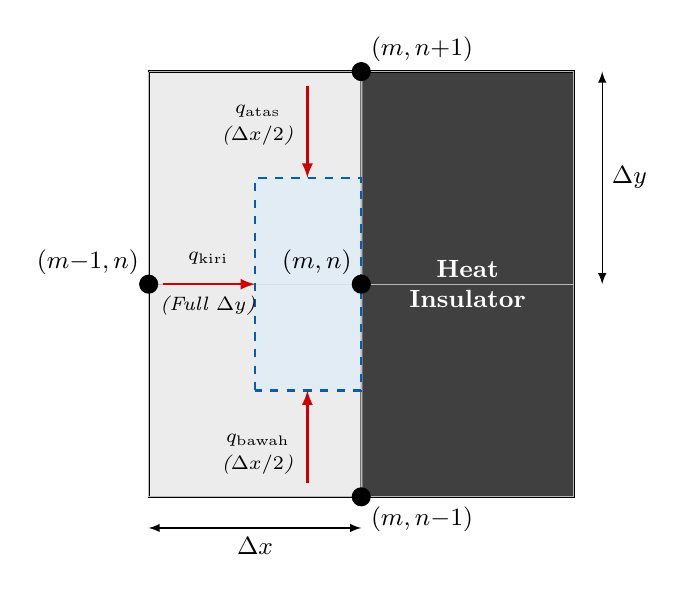
\begin{tikzpicture}[scale=1.8, >=latex]
    \colorlet{metal}{gray!15}
    \colorlet{insulator}{black!75}
    \fill[metal]     (-1.5,-1.5) rectangle (0.0, 1.5);
    \fill[insulator] ( 0.0,-1.5) rectangle (1.5, 1.5);
    \node[white, font=\small\bfseries, align=center] at (0.75,0) {Heat\\Insulator};
    \draw[black, thick] (-1.5,-1.5) rectangle (1.5,1.5);
    \draw[black!55, very thick] (0,-1.5) -- (0,1.5);
    \foreach \x in {-1.5, 0, 1.5} \draw[gray!55, thin] (\x,-1.5) -- (\x,1.5);
    \foreach \y in {-1.5, 0, 1.5} \draw[gray!55, thin] (-1.5,\y) -- (1.5,\y);
    \draw[dashed, thick, itbblue, fill=itbblue!12, fill opacity=0.8] (-0.75,-0.75) rectangle (0.00,0.75);
    
    \draw[<->, thin, black] (-1.5,-1.72) -- (0,-1.72) node[midway, below, font=\small] {$\Delta x$};
    \draw[<->, thin, black] (1.7,0) -- (1.7,1.5) node[midway, right, font=\small] {$\Delta y$};
    
    \draw[->, thick, red!80!black] (-1.40, 0.0) -- (-0.75, 0.0);
    \node[font=\scriptsize, black] at (-1.08, 0.18) {$q_\text{kiri}$};
    \node[font=\scriptsize, black] at (-1.08, -0.15) {\textit{(Full $\Delta y$)}};
    
    \draw[->, thick, red!80!black] (-0.38, 1.40) -- (-0.38, 0.75);
    \node[font=\scriptsize, black] at (-0.73, 1.22) {$q_\text{atas}$};
    \node[font=\scriptsize, black] at (-0.73, 1.05) {\textit{($\Delta x/2$)}};
    
    \draw[->, thick, red!80!black] (-0.38, -1.40) -- (-0.38, -0.75);
    \node[font=\scriptsize, black] at (-0.73, -1.10) {$q_\text{bawah}$};
    \node[font=\scriptsize, black] at (-0.73, -1.27) {\textit{($\Delta x/2$)}};
    
    \filldraw[black] ( 0.0,  0.0) circle (1.8pt) node[above left, font=\small] {$(m,n)$};
    \filldraw[black] (-1.5,  0.0) circle (1.8pt) node[above left,  font=\small] {$(m{-}1,n)$};
    \filldraw[black] ( 0.0,  1.5) circle (1.8pt) node[above right,  font=\small] {$(m,n{+}1)$};
    \filldraw[black] ( 0.0, -1.5) circle (1.8pt) node[below right,  font=\small] {$(m,n{-}1)$};
\end{tikzpicture}
\caption{Visualisasi \textit{control volume} pada permukaan datar batas isolator $(m,n)$. Sisi kanan tidak menerima fluks akibat dinding adiabatik ($q_{\text{kanan}} = 0$).}
\label{fig:kasus_2}
\end{figure}

Sebagai contoh, untuk \textit{node} di tepi kiri isolator, fluks konduksi dijabarkan menggunakan Hukum Fourier ($q = k \cdot A \cdot \frac{\Delta T}{L}$) dengan asumsi ketebalan benda $1\text{ m}$:
\begin{align*}
    q_{\text{kiri}}  &= k \cdot (\Delta y \cdot 1) \cdot \frac{T_{m-1,n} - T_{m,n}}{\Delta x} \\
    q_{\text{atas}}  &= k \cdot \left(\frac{\Delta x}{2} \cdot 1\right) \cdot \frac{T_{m,n+1} - T_{m,n}}{\Delta y} \\
    q_{\text{bawah}} &= k \cdot \left(\frac{\Delta x}{2} \cdot 1\right) \cdot \frac{T_{m,n-1} - T_{m,n}}{\Delta y} \\
    q_{\text{kanan}} &= 0 \quad \text{(Dinding adiabatik isolator)}
\end{align*}
Mensubstitusi keempat persamaan tersebut ke kesetimbangan energi ($\sum q = 0$):
\begin{equation}
    k \Delta y \frac{T_{m-1,n} - T_{m,n}}{\Delta x} + k \frac{\Delta x}{2} \frac{T_{m,n+1} - T_{m,n}}{\Delta y} + k \frac{\Delta x}{2} \frac{T_{m,n-1} - T_{m,n}}{\Delta y} = 0
\end{equation}
Terapkan kondisi $\Delta x = \Delta y$, sehingga suku pembagi spasial akan bernilai 1 ($\frac{\Delta y}{\Delta x} = 1$ dan $\frac{\Delta x}{\Delta y} = 1$):
\begin{equation}
    k \big(T_{m-1,n} - T_{m,n}\big) + \frac{k}{2} \big(T_{m,n+1} - T_{m,n}\big) + \frac{k}{2} \big(T_{m,n-1} - T_{m,n}\big) = 0
\end{equation}
Bagi seluruh ruas dengan $\frac{k}{2}$ untuk menyederhanakan pecahan:
\begin{equation}
    2 \big(T_{m-1,n} - T_{m,n}\big) + 1 \big(T_{m,n+1} - T_{m,n}\big) + 1 \big(T_{m,n-1} - T_{m,n}\big) = 0
\end{equation}
\begin{equation}
    2T_{m-1,n} + T_{m,n+1} + T_{m,n-1} - 4T_{m,n} = 0
\end{equation}
Maka diperoleh persamaan akhir titik permukaan datar isolator:
\begin{equation} \label{eq:insulator_flat_final}
    T_{m,n} = \frac{2T_{m-1,n} + T_{m,n+1} + T_{m,n-1}}{4}
\end{equation}

\subsubsection*{Kasus 3: Node Sudut Dalam Isolator}
Untuk titik di sudut dalam ruang isolator (misalnya pada pojok kiri-atas isolator pada Gambar~\ref{fig:kasus_3}), material solid mengelilingi \textit{node} sebesar $3/4$ luasan. Metode Kesetimbangan Energi kembali diterapkan.

\begin{figure}[h!]
\centering
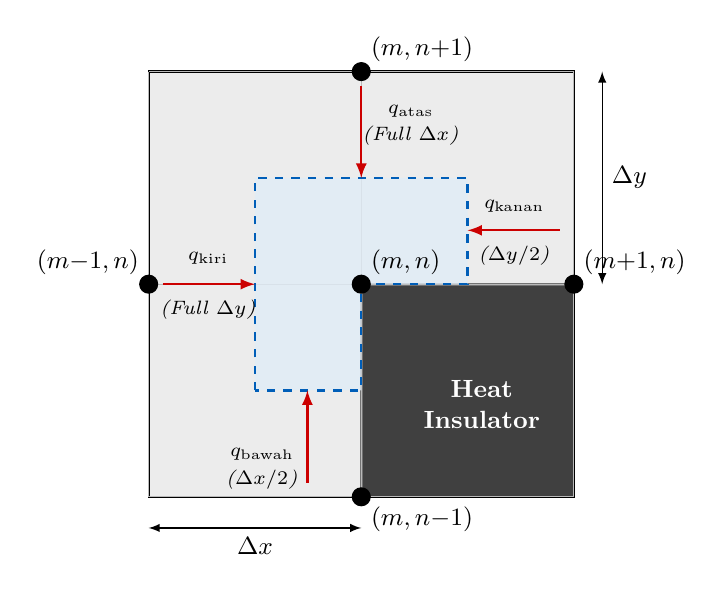
\begin{tikzpicture}[scale=1.8, >=latex]
    \colorlet{metal}{gray!15}
    \colorlet{insulator}{black!75}
    \fill[metal]     (-1.5,-1.5) rectangle (1.5, 1.5);
    \fill[insulator] ( 0.0,-1.5) rectangle (1.5, 0.0);
    \node[white, font=\small\bfseries, align=center] at (0.85,-0.85) {Heat\\Insulator};
    \draw[black, thick] (-1.5,-1.5) rectangle (1.5,1.5);
    \draw[black!55, very thick] (0,0) -- (1.5,0);
    \draw[black!55, very thick] (0,0) -- (0,-1.5);
    \foreach \x in {-1.5, 0, 1.5} \draw[gray!55, thin] (\x,-1.5) -- (\x,1.5);
    \foreach \y in {-1.5, 0, 1.5} \draw[gray!55, thin] (-1.5,\y) -- (1.5,\y);
    \draw[dashed, thick, itbblue, fill=itbblue!12, fill opacity=0.8]
        (-0.75,-0.75) -- (-0.75, 0.75) -- (0.75, 0.75) --
        (0.75,  0.00) -- ( 0.00, 0.00) -- (0.00,-0.75) -- cycle;
        
    \draw[<->, thin, black] (-1.5,-1.72) -- (0,-1.72) node[midway, below, font=\small] {$\Delta x$};
    \draw[<->, thin, black] (1.7,0) -- (1.7,1.5) node[midway, right, font=\small] {$\Delta y$};
    
    \draw[->, thick, red!80!black] (-1.40, 0.0) -- (-0.75, 0.0);
    \node[font=\scriptsize, black] at (-1.08, 0.18) {$q_\text{kiri}$};
    \node[font=\scriptsize, black, align=center] at (-1.08, -0.18) {\textit{(Full $\Delta y$)}};
    
    \draw[->, thick, red!80!black] (0.0, 1.40) -- (0.0, 0.75);
    \node[font=\scriptsize, black] at (0.35, 1.22) {$q_\text{atas}$};
    \node[font=\scriptsize, black] at (0.35, 1.05) {\textit{(Full $\Delta x$)}};
    
    \draw[->, thick, red!80!black] (1.40, 0.38) -- (0.75, 0.38);
    \node[font=\scriptsize, black] at (1.08, 0.55) {$q_\text{kanan}$};
    \node[font=\scriptsize, black] at (1.08, 0.20) {\textit{($\Delta y/2$)}};
    
    \draw[->, thick, red!80!black] (-0.38,-1.40) -- (-0.38,-0.75);
    \node[font=\scriptsize, black] at (-0.70,-1.20) {$q_\text{bawah}$};
    \node[font=\scriptsize, black] at (-0.70,-1.38) {\textit{($\Delta x/2$)}};
    
    \filldraw[black] ( 0.0,  0.0) circle (1.8pt) node[above right, font=\small] {$(m,n)$};
    \filldraw[black] (-1.5,  0.0) circle (1.8pt) node[above left,  font=\small] {$(m{-}1,n)$};
    \filldraw[black] ( 1.5,  0.0) circle (1.8pt) node[above right, font=\small] {$(m{+}1,n)$};
    \filldraw[black] ( 0.0,  1.5) circle (1.8pt) node[above right, font=\small] {$(m,n{+}1)$};
    \filldraw[black] ( 0.0, -1.5) circle (1.8pt) node[below right, font=\small] {$(m,n{-}1)$};
\end{tikzpicture}
\caption{Visualisasi \textit{control volume} berbentuk-L pada titik sudut dalam isolator $(m,n)$.}
\label{fig:kasus_3}
\end{figure}

Aliran fluks konduksinya dijabarkan sebagai:
\begin{align*}
    q_{\text{kiri}}  &= k \cdot (\Delta y) \cdot \frac{T_{m-1,n} - T_{m,n}}{\Delta x} \\
    q_{\text{atas}}  &= k \cdot (\Delta x) \cdot \frac{T_{m,n+1} - T_{m,n}}{\Delta y} \\
    q_{\text{kanan}} &= k \cdot \left(\frac{\Delta y}{2}\right) \cdot \frac{T_{m+1,n} - T_{m,n}}{\Delta x} \\
    q_{\text{bawah}} &= k \cdot \left(\frac{\Delta x}{2}\right) \cdot \frac{T_{m,n-1} - T_{m,n}}{\Delta y}
\end{align*}
Substitusi ke dalam kesetimbangan energi ($\sum q = 0$):
\begin{equation}
    k \Delta y \frac{T_{m-1,n} - T_{m,n}}{\Delta x} + k \Delta x \frac{T_{m,n+1} - T_{m,n}}{\Delta y} + k \frac{\Delta y}{2} \frac{T_{m+1,n} - T_{m,n}}{\Delta x} + k \frac{\Delta x}{2} \frac{T_{m,n-1} - T_{m,n}}{\Delta y} = 0
\end{equation}
Terapkan kondisi $\Delta x = \Delta y$:
\begin{equation}
    k \big(T_{m-1,n} - T_{m,n}\big) + k \big(T_{m,n+1} - T_{m,n}\big) + \frac{k}{2} \big(T_{m+1,n} - T_{m,n}\big) + \frac{k}{2} \big(T_{m,n-1} - T_{m,n}\big) = 0
\end{equation}
Untuk menghilangkan pecahan pada ruas, bagi seluruh komponen dengan $\frac{k}{2}$:
\begin{equation}
    2 \big(T_{m-1,n} - T_{m,n}\big) + 2 \big(T_{m,n+1} - T_{m,n}\big) + 1 \big(T_{m+1,n} - T_{m,n}\big) + 1 \big(T_{m,n-1} - T_{m,n}\big) = 0
\end{equation}
\begin{equation}
    2T_{m-1,n} + 2T_{m,n+1} + T_{m+1,n} + T_{m,n-1} - 6T_{m,n} = 0
\end{equation}
Sehingga formulasi akhir titik sudut isolator diselesaikan menjadi:
\begin{equation} \label{eq:insulator_corner_final}
    T_{m,n} = \frac{2T_{m-1,n} + 2T_{m,n+1} + T_{m+1,n} + T_{m,n-1}}{6}
\end{equation}

% --- SUBSECTION: Metode Penyelesaian Numerik ---
\subsection{Metode Penyelesaian Numerik: Iterasi Gauss-Seidel}
Diskritisasi persamaan diferensial parsial pada seluruh jaringan kisi (\textit{grid}) domain pelat 2D akan menghasilkan sebuah Sistem Persamaan Linier Aljabar (SPLA) yang sangat besar. Untuk ukuran grid yang masif, penyelesaian analitis (seperti inversi matriks langsung) membutuhkan alokasi memori komputer yang sangat besar dan rawan terhadap galat pembulatan (\textit{round-off error}). Oleh karena itu, SPLA pada tugas ini diselesaikan menggunakan pendekatan komputasi numerik iteratif.

Metode numerik yang dipilih dan umum digunakan untuk menyelesaikan kasus perpindahan panas kondisi tunak ini adalah \textbf{Metode Iterasi Gauss-Seidel}. Pemilihan metode ini didasarkan pada dua keunggulan utama dibandingkan metode iterasi standar lainnya (seperti metode Jacobi):
\begin{enumerate}
    \item \textbf{Tingkat Konvergensi yang Lebih Cepat:} Pada metode Gauss-Seidel, nilai temperatur terbaru yang baru saja dihitung pada suatu \textit{node} akan langsung digunakan untuk menghitung temperatur \textit{node} tetangga di sebelahnya pada langkah iterasi yang sama. Pembaruan nilai secara instan ini membuat laju konvergensi Gauss-Seidel secara umum dua kali lebih cepat daripada metode Jacobi (yang harus menunggu seluruh \textit{grid} selesai dihitung sebelum nilainya diperbarui).
    \item \textbf{Efisiensi Memori:} Karena nilai lama langsung ditimpa (\textit{overwrite}) oleh nilai baru pada saat komputasi berlangsung, program tidak perlu mengalokasikan matriks memori ganda untuk menyimpan status temperatur dari iterasi sebelumnya secara keseluruhan.
\end{enumerate}

\paragraph{Algoritma Komputasi.} 
Proses eksekusi algoritma Gauss-Seidel pada simulasi ini mengikuti tahapan matematis berikut:
\begin{enumerate}
    \item \textbf{Inisialisasi (\textit{Initial Guess}):} Seluruh titik \textit{interior} dan batas isolator diberikan nilai tebakan awal ($T_{m,n}^{(0)}$). Kondisi batas Dirichlet (sisi luar pelat) ditetapkan pada nilai suhu konstan sesuai spesifikasi soal dan tidak ikut diiterasi.
    \item \textbf{Penyapuan Ruang (\textit{Spatial Sweep}):} Program melakukan iterasi (menyapu \textit{node} demi \textit{node}) secara berurutan, misalnya dari kiri-atas ke kanan-bawah. Nilai temperatur baru dihitung berdasarkan persamaan kesetimbangan fisis yang telah diturunkan (Kasus 1, Kasus 2, atau Kasus 3).
    \item \textbf{Evaluasi Konvergensi:} Setelah satu siklus penyapuan matriks selesai, program akan menghitung nilai \textit{error residual} absolut maksimum antara iterasi saat ini ($i$) dan iterasi sebelumnya ($i-1$).
\end{enumerate}
Proses iterasi ini akan terus diulang hingga sistem mencapai kondisi stabil, yang ditandai dengan terpenuhinya kriteria toleransi konvergensi:
\begin{equation}
    |T_{m,n}^{(i)} - T_{m,n}^{(i-1)}|_{\text{maks}} \leq \epsilon
\end{equation}
di mana $\epsilon$ adalah batas toleransi galat yang sangat kecil (misalnya $\epsilon = 10^{-5}$).

% ============================================================
%  SUBSECTION: Contoh Perhitungan Iterasi Manual (Gauss-Seidel)
% ============================================================

\subsection{Contoh Perhitungan Iterasi Manual (Metode Gauss-Seidel)}
Untuk memberikan gambaran matematis mengenai proses yang dieksekusi oleh program komputasi, berikut disajikan contoh perhitungan manual satu langkah iterasi Gauss-Seidel. Sesuai dengan struktur algoritma kondisional pada \textit{script} MATLAB, evaluasi dilakukan dari kondisi geometri yang paling spesifik hingga yang paling umum untuk menghindari tumpang tindih (\textit{overlapping}) identifikasi \textit{node}.

Dalam implementasinya, program menggunakan tebakan awal rata-rata $T^{(0)} = 47.5^\circ\text{C}$ untuk seluruh titik guna mempercepat konvergensi. Namun, untuk keperluan ilustrasi perhitungan manual ini, akan digunakan nilai-nilai tebakan awal hipotetis yang bervariasi agar proses rata-rata pembobotannya terlihat lebih jelas.

% ----------------------------------------------------------
%  KASUS 3: NODE SUDUT DALAM ISOLATOR
% ----------------------------------------------------------
\subsubsection*{1. Eksekusi Kasus 3: Node Sudut Dalam Isolator}
Kondisi ini merupakan evaluasi paling spesifik (merujuk pada \texttt{elseif i == i1 \&\& j == j2} di dalam \textit{script} untuk pojok kiri-atas isolator). Pada iterasi Gauss-Seidel, nilai \textit{node} di sebelah kiri dan atas diasumsikan telah diperbarui karena urutan penyapuan matriks (\textit{sweep}) umumnya bergerak searah indeks. Formulasinya mengacu pada Persamaan (\ref{eq:insulator_corner_final}).

\paragraph{Kondisi Awal (Iterasi ke-0):}
\begin{center}
\renewcommand{\arraystretch}{1.2}
\begin{tabular}{|c|l|c|c|}
\hline
\textbf{Node} & \textbf{Posisi Relatif (Pembobot)} & \textbf{Status Nilai} & \textbf{Temperatur ($^\circ$C)} \\
\hline
$T_{m-1,n}$ & Kiri (Penuh, bobot 2) & Diperbarui ($i=1$) & $80.00$ \\
$T_{m,n+1}$ & Atas (Penuh, bobot 2) & Diperbarui ($i=1$) & $60.00$ \\
$T_{m+1,n}$ & Kanan (Setengah, bobot 1) & Tebakan Lama ($i=0$) & $40.00$ \\
$T_{m,n-1}$ & Bawah (Setengah, bobot 1) & Tebakan Lama ($i=0$) & $50.00$ \\
\hline
\multicolumn{3}{|l|}{Total Pembagi} & $\mathbf{6}$ \\
\hline
\end{tabular}
\end{center}

\paragraph{Perhitungan Iterasi 1 ($i = 1$):}
\begin{align*}
T_{m,n}^{(1)}
    &= \frac{2\,T_{m-1,n}^{(1)} + 2\,T_{m,n+1}^{(1)} + T_{m+1,n}^{(0)} + T_{m,n-1}^{(0)}}{6} \\[4pt]
    &= \frac{2(80.00) + 2(60.00) + 40.00 + 50.00}{6} \\[4pt]
    &= \frac{160.00 + 120.00 + 40.00 + 50.00}{6} = \frac{370.00}{6} = \boxed{61.67^\circ\text{C}}
\end{align*}

% ----------------------------------------------------------
%  KASUS 2: NODE PERMUKAAN DATAR ISOLATOR
% ----------------------------------------------------------
\subsubsection*{2. Eksekusi Kasus 2: Node Permukaan Datar Isolator}
Jika titik komputasi tidak berada persis di sudut, program akan mengevaluasi apakah titik tersebut berada di sepanjang tepi datar isolator (merujuk pada kondisi \texttt{elseif i == i1 \&\& j > j1 \&\& j < j2} untuk tepi kiri isolator). Formulasinya dieksekusi menggunakan Persamaan (\ref{eq:insulator_flat_final}). Sisi kanan diabaikan dari perhitungan karena fluks bernilai nol.

\paragraph{Kondisi Awal (Iterasi ke-0):}
\begin{center}
\renewcommand{\arraystretch}{1.2}
\begin{tabular}{|c|l|c|c|}
\hline
\textbf{Node} & \textbf{Posisi Relatif (Pembobot)} & \textbf{Status Nilai} & \textbf{Temperatur ($^\circ$C)} \\
\hline
$T_{m-1,n}$ & Kiri (Penuh, bobot 2) & Diperbarui ($i=1$) & $65.00$ \\
$T_{m,n+1}$ & Atas (Setengah, bobot 1) & Diperbarui ($i=1$) & $55.00$ \\
$T_{m,n-1}$ & Bawah (Setengah, bobot 1) & Tebakan Lama ($i=0$) & $45.00$ \\
\hline
\multicolumn{3}{|l|}{Total Pembagi} & $\mathbf{4}$ \\
\hline
\end{tabular}
\end{center}

\paragraph{Perhitungan Iterasi 1 ($i = 1$):}
\begin{align*}
T_{m,n}^{(1)}
    &= \frac{2\,T_{m-1,n}^{(1)} + T_{m,n+1}^{(1)} + T_{m,n-1}^{(0)}}{4} \\[4pt]
    &= \frac{2(65.00) + 55.00 + 45.00}{4} \\[4pt]
    &= \frac{130.00 + 55.00 + 45.00}{4} = \frac{230.00}{4} = \boxed{57.50^\circ\text{C}}
\end{align*}

% ----------------------------------------------------------
%  KASUS 1: NODE INTERIOR
% ----------------------------------------------------------
\subsubsection*{3. Eksekusi Kasus 1: Node Interior}
Apabila \textit{node} yang dievaluasi tidak termasuk ke dalam kategori isolator maupun sudutnya, algoritma \textit{script} akan mengeksekusi blok \texttt{else} yang paling umum, yaitu titik interior biasa. Titik ini menerima konduksi seragam dari keempat arah, sehingga pembobotannya adalah rata-rata aritmatika murni.

\paragraph{Kondisi Awal (Iterasi ke-0):}
\begin{center}
\renewcommand{\arraystretch}{1.2}
\begin{tabular}{|c|l|c|c|}
\hline
\textbf{Node} & \textbf{Posisi Relatif (Pembobot)} & \textbf{Status Nilai} & \textbf{Temperatur ($^\circ$C)} \\
\hline
$T_{m-1,n}$ & Kiri (Penuh, bobot 1) & Diperbarui ($i=1$) & $60.00$ \\
$T_{m,n+1}$ & Atas (Penuh, bobot 1) & Diperbarui ($i=1$) & $55.00$ \\
$T_{m+1,n}$ & Kanan (Penuh, bobot 1) & Tebakan Lama ($i=0$) & $35.00$ \\
$T_{m,n-1}$ & Bawah (Penuh, bobot 1) & Tebakan Lama ($i=0$) & $40.00$ \\
\hline
\multicolumn{3}{|l|}{Total Pembagi} & $\mathbf{4}$ \\
\hline
\end{tabular}
\end{center}

\paragraph{Perhitungan Iterasi 1 ($i = 1$):}
\begin{align*}
T_{m,n}^{(1)}
    &= \frac{T_{m-1,n}^{(1)} + T_{m+1,n}^{(0)} + T_{m,n+1}^{(1)} + T_{m,n-1}^{(0)}}{4} \\[4pt]
    &= \frac{60.00 + 35.00 + 55.00 + 40.00}{4} \\[4pt]
    &= \frac{190.00}{4} = \boxed{47.50^\circ\text{C}}
\end{align*}

\vspace{0.3cm}
Ketiga proses komputasi di atas dieksekusi secara masif di dalam matriks \texttt{T(Nx, Ny)} oleh program MATLAB. Nilai \textit{node} yang baru saja didapatkan (misal $57.50^\circ\text{C}$ pada Kasus 2) akan langsung digunakan pada hitungan titik sebelahnya dalam langkah iterasi yang sama. Proses ini terus berulang (\textit{while loop}) hingga selisih nilai suhu absolut maksimum pada seluruh matriks berada di bawah kriteria toleransi galat (\texttt{err < tol}).

% ----------------------------------------------------------
%  EVALUASI KONVERGENSI / ERROR
% ----------------------------------------------------------
\subsubsection*{4. Evaluasi Kriteria Konvergensi (\textit{Residual Error})}
Ketiga proses komputasi di atas dieksekusi secara masif di dalam matriks jaringan spasial \texttt{T(Nx, Ny)} oleh program MATLAB. Nilai \textit{node} yang baru saja didapatkan akan langsung ditimpa (\textit{overwrite}) dan digunakan pada perhitungan titik di sebelahnya dalam langkah penyapuan (\textit{sweep}) matriks yang sama.

Untuk menentukan kapan iterasi (\textit{looping}) ini harus dihentikan, program menggunakan kriteria konvergensi berdasarkan evaluasi \textbf{Galat Residu Absolut Maksimum (\textit{Maximum Absolute Residual Error})}. Iterasi dianggap telah mencapai kondisi stabil (tunak) apabila selisih perubahan suhu terbesar di seluruh titik matriks antara iterasi saat ini ($i$) dan iterasi sebelumnya ($i-1$) sudah lebih kecil dari batas toleransi yang ditetapkan ($\epsilon$).

Secara matematis, kriteria penghentian komputasi ini dirumuskan sebagai:
\begin{equation} \label{eq:error}
    \text{Error} = \max \left| T_{m,n}^{(i)} - T_{m,n}^{(i-1)} \right| \leq \epsilon
\end{equation}

Untuk pemodelan distribusi temperatur dengan rentang suhu $20^\circ\text{C}$ hingga $100^\circ\text{C}$, nilai toleransi galat (\text{tol}) yang umum dan ideal digunakan adalah $\epsilon = 10^{-4}$ atau $\epsilon = 10^{-5}$. Nilai ini menjamin bahwa fluktuasi komputasi sudah berada di angka desimal yang tidak lagi signifikan secara fisis.

\paragraph{Contoh Perhitungan Evaluasi Error:}
Mengambil data dari perhitungan manual \textbf{Kasus 3 (Node Sudut Dalam Isolator)} di atas, mari kita evaluasi apakah komputasi sudah boleh dihentikan pada Iterasi ke-1.
\begin{itemize}
    \item Nilai pada Iterasi ke-0 (Tebakan awal) : $T_{m,n}^{(0)} = 47.50^\circ\text{C}$ \textit{(Asumsi rata-rata suhu awal keseluruhan program)}
    \item Nilai pada Iterasi ke-1 (Hasil hitung) : $T_{m,n}^{(1)} = 61.67^\circ\text{C}$
\end{itemize}
Maka besar *error* pada titik sudut tersebut untuk iterasi pertama adalah:
\begin{align*}
    e_{m,n}^{(1)} &= \left| T_{m,n}^{(1)} - T_{m,n}^{(0)} \right| \\
    e_{m,n}^{(1)} &= \left| 61.67 - 47.50 \right| = 14.17^\circ\text{C}
\end{align*}
Karena nilai galat komputasi $14.17 > 10^{-4}$, maka kriteria konvergensi pada Persamaan (\ref{eq:error}) belum terpenuhi. Oleh karena itu, program (seperti pada \textit{script while-loop} MATLAB) akan memutus perulangan ini belum selesai dan secara otomatis akan melanjutkan ke perhitungan Iterasi ke-2, ke-3, dan seterusnya hingga $e_{m,n}^{(i)} \leq 10^{-4}$ terpenuhi di semua titik.

% --- SECTION 4: HASIL DAN PEMBAHASAN ---
\section{Hasil dan Pembahasan}
Berdasarkan formulasi diskritisasi yang telah diturunkan sebelumnya, simulasi komputasional dijalankan menggunakan perangkat lunak MATLAB. Analisis difokuskan pada dua aspek utama yaitu variasi material logam dan pengaruh ukuran kisi (resolusi grid) spasial.

\subsection{Analisis Variasi Material Logam}
Simulasi ini membandingkan dua jenis material logam yang umum digunakan dalam aplikasi keteknikan, yaitu Tembaga (konduktor termal sangat baik) dan Baja Karbon (konduktor termal menengah). Properti fisis yang digunakan ditunjukkan pada Tabel 1.

\begin{table}[h!]
\centering
\caption{Properti Termal Variasi Material Logam \cite{incropera_principles_2013}}
\renewcommand{\arraystretch}{1.25}
\begin{tabular}{|c|p{0.38\textwidth}|p{0.20\textwidth}|p{0.20\textwidth}|}
\hline
\textbf{No} & \centering\textbf{Jenis Logam} & \centering\textbf{Konduktivitas Termal ($k$)} & \centering\arraybackslash\textbf{Sifat Termal} \\
\hline
1 & Tembaga (\textit{Copper}, murni) & $401\text{ W/m}\cdot\text{K}$ & Konduktor Tinggi \\
\hline
2 & Baja Karbon (\textit{Carbon Steel} 1\%) & $43\text{ W/m}\cdot\text{K}$ & Konduktor Sedang \\
\hline
\end{tabular}
\end{table}

Berdasarkan hasil eksekusi program, distribusi temperatur kondisi tunak (\textit{steady-state}) untuk Tembaga dan Baja Karbon menunjukkan \textbf{profil kontur dan gradien spasial yang sama persis}. Fenomena ini dapat dibuktikan secara matematis melalui reduksi persamaan pembangunnya. Berangkat dari persamaan difusi kalor 2D kondisi tunak, di mana konduktivitas termal ($k$) diasumsikan konstan dan dapat difaktorkan keluar dari turunan:
\begin{equation}
    k \left( \frac{\partial^2 T}{\partial x^2} + \frac{\partial^2 T}{\partial y^2} \right) + \dot{q} = 0
\end{equation}

Karena pada material pelat diasumsikan tidak ada sumber pembangkitan panas internal ($\dot{q} = 0$), persamaan di atas menjadi:
\begin{equation}
    k \left( \frac{\partial^2 T}{\partial x^2} + \frac{\partial^2 T}{\partial y^2} \right) = 0
\end{equation}

Mengingat nilai properti konduktivitas termal material fisis tidak mungkin bernilai nol ($k \neq 0$), kita dapat membagi kedua ruas dengan nilai $k$ sehingga variabel tersebut saling menghilangkan (\textit{dicoret}). Hal ini mereduksi sistem murni menjadi Persamaan Laplace:
\begin{equation} \label{eq:laplace_reduced}
    \frac{\partial^2 T}{\partial x^2} + \frac{\partial^2 T}{\partial y^2} = 0 \quad \Longrightarrow \quad \nabla^2 T = 0
\end{equation}

Oleh karena itu, terbukti bahwa pada kondisi tunak murni tanpa \textit{heat generation}, distribusi spasial temperatur ($T$) dalam pelat \textbf{hanya bergantung pada geometri domain dan nilai kondisi batas Dirichlet}, dan sama sekali terbebas (independen) dari jenis materialnya.

Perbedaan properti konduktivitas termal ($k$) antara Tembaga dan Baja Karbon tidak akan teramati pada profil suhu, melainkan baru akan bermanifestasi pada besaran absolut \textbf{Laju Perpindahan Panas (Fluks Kalor, $q''$)}. Berdasarkan Hukum Fourier, magnitudo fluks kalor dirumuskan sebagai:
\begin{equation} \label{eq:fourier_flux}
    |\vec{q}''| = |-k \nabla T| = k \sqrt{ \left( \frac{\partial T}{\partial x} \right)^2 + \left( \frac{\partial T}{\partial y} \right)^2 }
\end{equation}

Untuk membuktikan hipotesis ini, komputasi gradien temperatur ($\nabla T$) dilakukan terhadap matriks suhu yang telah konvergen, lalu dikalikan dengan konstanta $k$ masing-masing material. Hasil pemetaan magnitudo fluks kalor divisualisasikan pada Gambar 5.

\begin{figure}[h!]
\centering

\includegraphics[width=1.0\textwidth]{figures/analisis_variasi_material.pdf}
\caption{Perbandingan magnitudo fluks kalor ($q''$) antara pelat Baja Karbon (kiri) dan Tembaga (kanan). Profil gradien identik, namun skala magnitudo (lihat \textit{colorbar}) berbeda signifikan.}
\label{fig:flux_comparison}
\end{figure}

Merujuk pada Gambar \ref{fig:flux_comparison}, secara visual lokasi konsentrasi perpindahan panas tertinggi (ditandai dengan warna merah pekat) identik untuk kedua material, yaitu terkonsentrasi di sekitar sudut isolator dan dekat dengan batas kondiri Dirichlet bersuhu tinggi ($100^\circ\text{C}$). 

Akan tetapi, analisis kuantitatif pada skala \textit{colorbar} menunjukkan perbedaan esensial. Meskipun profil gradien spasialnya ($\nabla T$) identik, magnitudo fluks kalor yang mengalir pada pelat tembaga mencapai nilai yang jauh lebih masif dibandingkan baja karbon. Rasio perbandingan fluks kalor maksimal tersebut sebanding dengan rasio konduktivitas termalnya:
\begin{equation}
    \frac{q''_{\text{Tembaga}}}{q''_{\text{Baja Karbon}}} = \frac{k_{\text{Tembaga}} \cdot |\nabla T|}{k_{\text{Baja Karbon}} \cdot |\nabla T|} = \frac{401}{43} \approx 9.33
\end{equation}
Hal ini membuktikan bahwa untuk mempertahankan profil temperatur yang identik pada geometri yang sama, material Tembaga mentransmisikan energi kalor rata-rata 9,33 kali lebih besar dibandingkan Baja Karbon pada setiap satuan waktu dan satuan luas penampangnya.

\subsection{Analisis Variasi Ukuran Kisi (\textit{Grid Independence Test})}
Untuk mengevaluasi sensitivitas numerik dan menemukan keseimbangan optimal antara akurasi model dan beban komputasi (\textit{computational cost}), simulasi dieksekusi dengan empat variasi resolusi spasial: grid kasar ($\Delta x = 0.100\text{ m}$), menengah ($\Delta x = 0.050\text{ m}$), halus ($\Delta x = 0.010\text{ m}$), dan sangat halus ($\Delta x = 0.001\text{ m}$). 

Visualisasi perbandingan kontur temperatur dari keempat resolusi disajikan pada Gambar \ref{fig:grid_comparison}, sedangkan kurva independensi kisi berdasarkan pemantauan suhu di \textit{probe point} $(0.75, 0.75)$ diplot pada skala logaritmik dalam Gambar \ref{fig:grid_curve}.

\begin{figure}[h!]
\centering
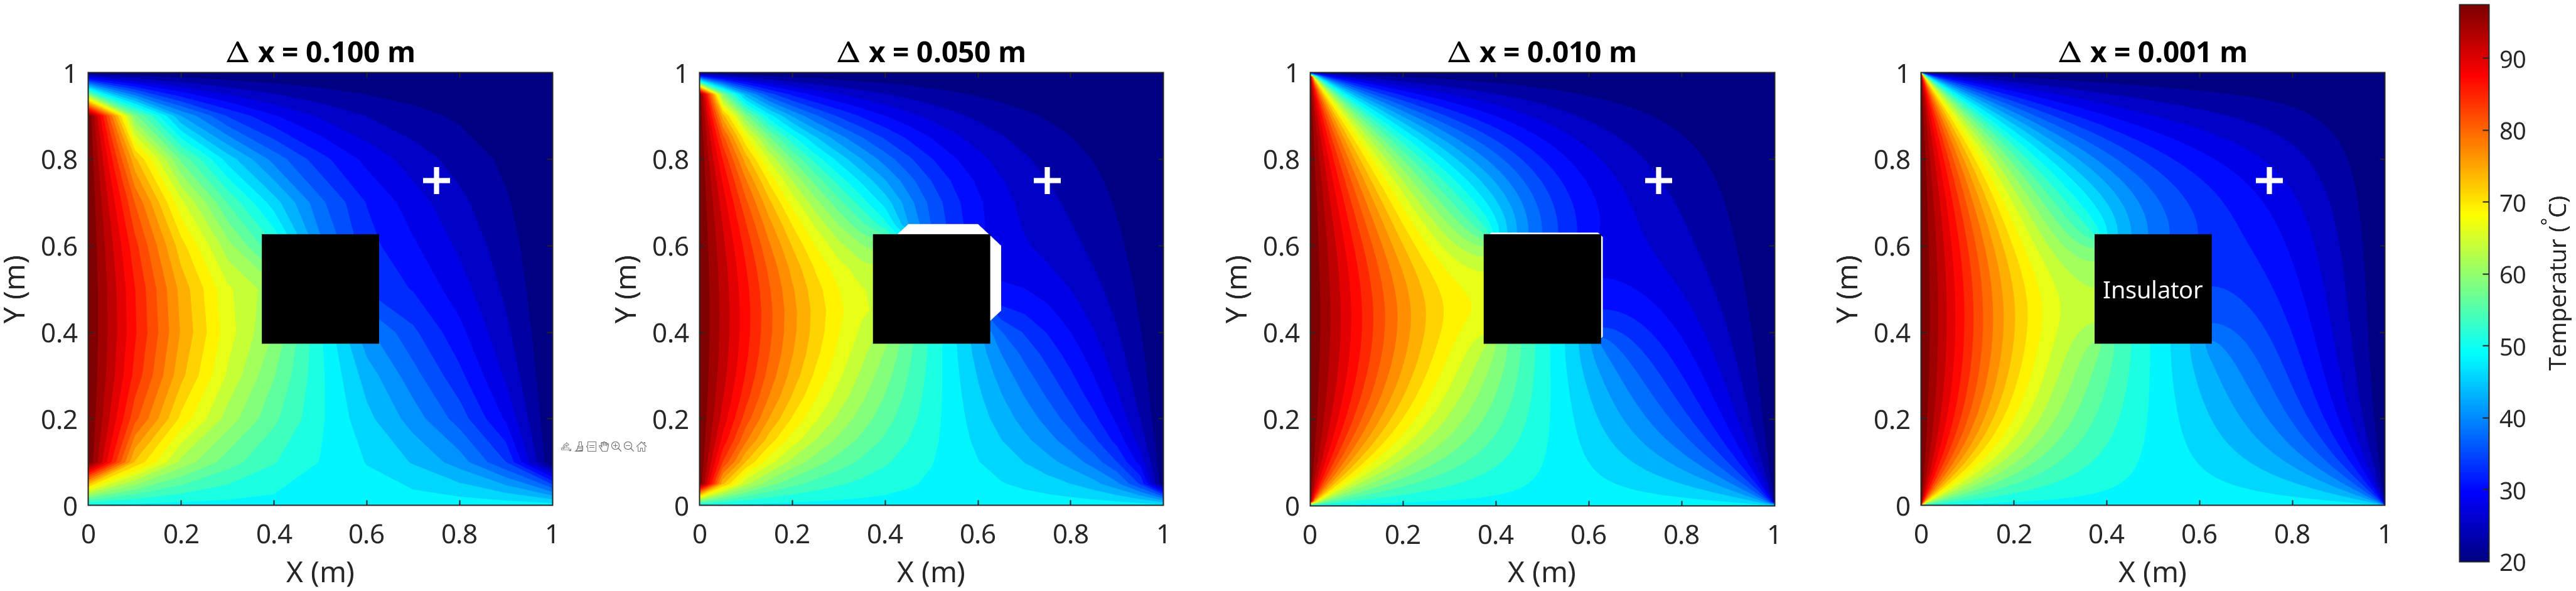
\includegraphics[width=1.0\textwidth]{figures/perbandingan_grid_kontur.png}
\caption{Perbandingan distribusi temperatur 2D pada berbagai resolusi kisi. \textit{Probe point} ditandai dengan simbol plus (+) putih di kuadran kanan atas.}
\label{fig:grid_comparison}
\end{figure}

\begin{figure}[h!]
\centering
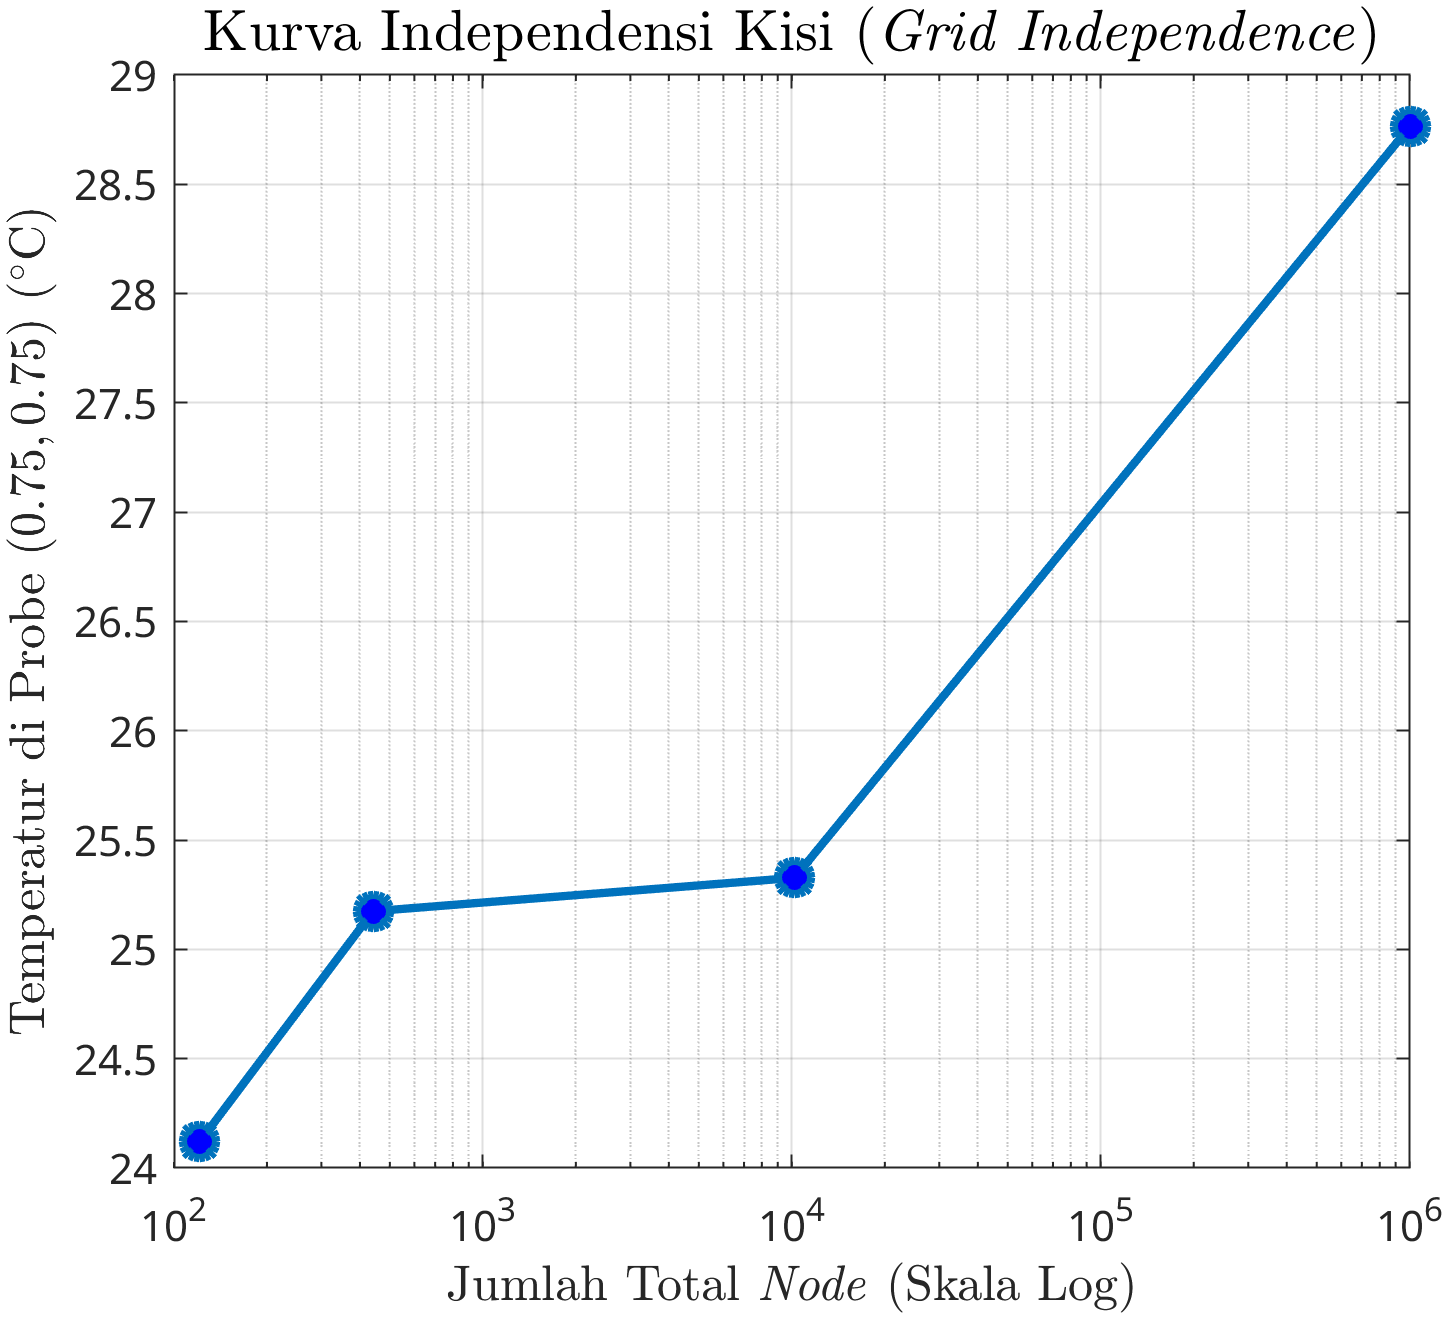
\includegraphics[width=0.7\textwidth]{figures/kurva_grid.png}
\caption{Kurva Independensi Kisi (\textit{Grid Independence}). Sumbu horizontal menggunakan skala logaritmik untuk merepresentasikan lompatan jumlah total \textit{node} komputasi hingga melampaui $10^6$ titik pada resolusi $\Delta x = 0.001\text{ m}$.}
\label{fig:grid_curve}
\end{figure}

Dari perbandingan keempat variasi resolusi grid tersebut, diperoleh analisis numerik komprehensif sebagai berikut:
\begin{enumerate}
    \item \textbf{Akurasi Visual dan Galat Geometri:} 
    Berdasarkan Gambar \ref{fig:grid_comparison}, penggunaan grid menengah ($\Delta x = 0.050\text{ m}$) memunculkan anomali galat geometri (\textit{geometrical truncation error}), terlihat dari adanya area putih di sekitar batas isolator. Hal ini terjadi karena batas fisis $0.375\text{ m}$ tidak dapat dibagi habis oleh kisi $0.050\text{ m}$, sehingga batas komputasi mengalami distorsi pembulatan. Sebaliknya, saat grid dirapatkan hingga $\Delta x = 0.001\text{ m}$, gradien warna menjadi sangat halus (\textit{high-fidelity}) dan batas geometri isolator terbentuk dengan presisi mutlak tanpa kebocoran spasial.

    \item \textbf{Stabilitas Nilai Fisis (\textit{Grid Convergence}):} 
    Pemantauan secara kuantitatif pada kurva Gambar \ref{fig:grid_curve} memberikan wawasan matematis yang krusial. Pada awalnya, transisi dari grid $0.050\text{ m}$ ke $0.010\text{ m}$ memberikan ilusi bahwa suhu telah mencapai konvergensi di kisaran $25.3^\circ\text{C}$. Namun, ketika resolusi dilipatgandakan secara ekstrem menjadi $0.001\text{ m}$ (lebih dari satu juta \textit{node}), nilai suhu terkoreksi secara signifikan mendekati $28.8^\circ\text{C}$. Hal ini membuktikan bahwa keberadaan singularitas pada sudut-sudut tajam isolator membutuhkan ukuran \textit{mesh} yang sangat padat agar terbebas sepenuhnya dari difusi numerik. Nilai pada kisi $0.001\text{ m}$ inilah yang merepresentasikan solusi fisis paling sejati.

    \item \textbf{Beban Komputasi dan \textit{Engineering Judgement}:} 
    Peningkatan resolusi dari $0.010\text{ m}$ ke $0.001\text{ m}$ memicu ledakan jumlah \textit{node} dari $10.201$ menjadi $1.002.001$ titik, yang secara langsung memperberat beban komputasi (\textit{computational cost}) secara eksponensial. Waktu eksekusi yang semula berada dalam skala sub-detik meningkat menjadi orde belasan menit. 
\end{enumerate}

Di dalam praktik komputasi teknik, penentuan ukuran kisi pada akhirnya kembali pada \textit{engineering judgement}—sebuah kompromi antara ketersediaan waktu dan tingkat akurasi yang dituntut oleh desain. Karena simulasi ini merupakan tahap analisis akhir (\textit{final reporting}) yang menuntut presisi mutlak tanpa toleransi galat geometri, \textbf{penulis memutuskan untuk memilih dan merekomendasikan kisi sangat halus $\Delta x = 0.001\text{ m}$}. Pengorbanan waktu komputasi selama belasan menit dinilai sangat rasional dan sepadan untuk mendapatkan resolusi \textit{high-fidelity} tertinggi yang sepenuhnya \textit{grid-independent}.

% --- SECTION 5: KESIMPULAN ---
\section{Kesimpulan}
Berdasarkan hasil simulasi komputasional dan analisis yang telah dilakukan, dapat ditarik beberapa kesimpulan utama sebagai berikut:
\begin{itemize}
    \item \textbf{Formulasi Diskritisasi dan Batas Isolator:} Pendekatan diferensial beda pusat dari Deret Taylor terbukti efektif untuk menyelesaikan titik interior logam yang kontinu. Namun, untuk titik pada antarmuka batas isolator termal (permukaan datar dan sudut), diskontinuitas material mengharuskan formulasi \textit{node} komputasi diturunkan secara fundamental menggunakan Metode Kesetimbangan Energi ($\sum q_{\text{in}} = 0$) guna mengkomodasi kondisi batas Neumann homogen.
    
    \item \textbf{Independensi Sifat Material pada Kondisi Tunak:} Pada kondisi tunak (\textit{steady-state}) tanpa adanya sumber pembangkitan panas internal ($\dot{q} = 0$), profil distribusi temperatur terbukti murni dikendalikan oleh geometri domain dan kondisi batas Dirichlet. Variabel konduktivitas termal material ($k$) saling mengeliminasi dalam Persamaan Laplace, sehingga pemilihan jenis logam (Tembaga maupun Baja Karbon) hanya memengaruhi besaran laju fluks kalor absolut ($q''$), bukan profil suhunya.
    
    \item \textbf{Efisiensi Solusi Numerik:} Metode iterasi Gauss-Seidel menunjukkan performa yang efisien dalam menyelesaikan Sistem Persamaan Linier Aljabar (SPLA) berukuran masif. Pembaruan nilai suhu tetangga secara instan (\textit{overwrite}) meminimalkan alokasi memori matriks ganda dan mempercepat laju konvergensi menuju kriteria toleransi \textit{residual error} yang ditetapkan ($\epsilon \leq 10^{-4}$).
    
    \item \textbf{Uji Independensi Kisi (\textit{Grid Independence}):} Analisis menunjukkan bahwa geometri sudut tajam pada area \textit{heat insulator} sangat rentan memicu galat geometri (\textit{geometrical truncation error}) dan difusi numerik pada kisi yang kasar. Representasi fisika termal dengan presisi \textit{high-fidelity} (sejati) baru tercapai ketika resolusi grid diperketat secara ekstrem hingga $\Delta x = 0.001\text{ m}$ (melibatkan lebih dari 1 juta \textit{node}). Keputusan untuk menggunakan grid sangat halus ini sangat beralasan dan esensial demi mencapai kondisi \textit{grid-independent}, meskipun berdampak pada lonjakan beban komputasi.
\end{itemize}

% --- DAFTAR PUSTAKA ---
\renewcommand{\refname}{Daftar Pustaka} 
\bibliographystyle{ieeetr} 
\bibliography{references} 

\newpage
% --- SECTION 6: LAMPIRAN SCRIPT ---
\section{Lampiran: Script Program}

Berikut adalah lampiran \textit{script} program komputasi yang ditulis menggunakan perangkat lunak MATLAB untuk menyelesaikan persamaan numerik Metode Beda-Hingga, memvisualisasikan data, dan melakukan analisis performa grid.

\subsection*{Lampiran 1: Script Analisis Variasi Material Logam (Fluks Kalor)}
\begin{lstlisting}[language=Matlab, basicstyle=\ttfamily\scriptsize, caption={BedaHingga\_AnalisisVariasiMaterial.m}]
% =========================================================================
% IK5025 - Analisis Variasi Material Logam (Fluks Kalor)
% Membuktikan bahwa k tidak mengubah profil T, tetapi mengubah Magnitudo q''
% =========================================================================

clear; clc; close all;

%% 1. PROSES SOLVER (Diringkas dari script sebelumnya)
L = 1.0; dx = 0.01; dy = dx;
Nx = round(L/dx) + 1; Ny = round(L/dy) + 1;
i1 = round(0.375/dx) + 1; i2 = round(0.625/dx) + 1;
j1 = round(0.375/dy) + 1; j2 = round(0.625/dy) + 1;

T = ones(Nx, Ny) * 47.5; 
T(1, :) = 100; T(Nx, :) = 20; T(:, 1) = 50; T(:, Ny) = 20;

tol = 1e-5; err = 1;
while err > tol
    T_old = T;
    for i = 2:Nx-1
        for j = 2:Ny-1
            if i > i1 && i < i2 && j > j1 && j < j2
                continue; 
            elseif i == i1 && j == j2
                T(i,j) = (2*T(i-1,j) + 2*T(i,j+1) + T(i+1,j) + T(i,j-1)) / 6;
            elseif i == i1 && j == j1
                T(i,j) = (2*T(i-1,j) + 2*T(i,j-1) + T(i+1,j) + T(i,j+1)) / 6;
            elseif i == i2 && j == j2
                T(i,j) = (2*T(i+1,j) + 2*T(i,j+1) + T(i-1,j) + T(i,j-1)) / 6;
            elseif i == i2 && j == j1
                T(i,j) = (2*T(i+1,j) + 2*T(i,j-1) + T(i-1,j) + T(i,j+1)) / 6;
            elseif i == i1 && j > j1 && j < j2
                T(i,j) = (2*T(i-1,j) + T(i,j+1) + T(i,j-1)) / 4;
            elseif i == i2 && j > j1 && j < j2
                T(i,j) = (2*T(i+1,j) + T(i,j+1) + T(i,j-1)) / 4;
            elseif j == j1 && i > i1 && i < i2
                T(i,j) = (2*T(i,j-1) + T(i+1,j) + T(i-1,j)) / 4;
            elseif j == j2 && i > i1 && i < i2
                T(i,j) = (2*T(i,j+1) + T(i+1,j) + T(i-1,j)) / 4;
            else
                T(i,j) = (T(i+1,j) + T(i-1,j) + T(i,j+1) + T(i,j-1)) / 4;
            end
        end
    end
    err = max(max(abs(T - T_old)));
end

% Hilangkan data di dalam isolator untuk proses gradien
T(i1+1:i2-1, j1+1:j2-1) = NaN;

%% 2. MENGHITUNG GRADIEN TEMPERATUR DAN FLUKS KALOR (HUKUM FOURIER)
[dTdy, dTdx] = gradient(T, dy, dx);

k_Cu = 401; % Tembaga
k_CS = 43;  % Baja Karbon

qx_Cu = -k_Cu * dTdx; qy_Cu = -k_Cu * dTdy;
qx_CS = -k_CS * dTdx; qy_CS = -k_CS * dTdy;

q_mag_Cu = sqrt(qx_Cu.^2 + qy_Cu.^2);
q_mag_CS = sqrt(qx_CS.^2 + qy_CS.^2);

%% 3. PLOTTING PERBANDINGAN FLUKS KALOR
x_lin = linspace(0, L, Nx); y_lin = linspace(0, L, Ny);
[X, Y] = meshgrid(x_lin, y_lin);

fig = figure('Color', 'w', 'Units', 'centimeters', 'Position', [2, 2, 28, 12]);

subplot(1,2,1);
contourf(X, Y, q_mag_CS', 25, 'LineColor', 'none');
colormap('hot'); 
c1 = colorbar; c1.Label.String = 'Fluks Kalor, q'''' (W/m^2)';
axis equal; axis tight;
title('Magnitudo Fluks Kalor: Baja Karbon (k = 43)', 'FontSize', 12);
xlabel('Jarak X (m)'); ylabel('Jarak Y (m)');
hold on;
rectangle('Position', [0.375, 0.375, 0.25, 0.25], 'FaceColor', 'k');
text(0.5, 0.5, 'Insulator', 'Color', 'w', 'HorizontalAlignment', 'center');
hold off;

subplot(1,2,2);
contourf(X, Y, q_mag_Cu', 25, 'LineColor', 'none');
colormap('hot'); 
c2 = colorbar; c2.Label.String = 'Fluks Kalor, q'''' (W/m^2)';
axis equal; axis tight;
title('Magnitudo Fluks Kalor: Tembaga (k = 401)', 'FontSize', 12);
xlabel('Jarak X (m)'); ylabel('Jarak Y (m)');
hold on;
rectangle('Position', [0.375, 0.375, 0.25, 0.25], 'FaceColor', 'k');
text(0.5, 0.5, 'Insulator', 'Color', 'w', 'HorizontalAlignment', 'center');
hold off;

set(fig, 'PaperUnits', 'centimeters');
set(fig, 'PaperSize', [28 12]);
set(fig, 'PaperPosition', [0 0 28 12]);

fprintf('Analisis Selesai');
\end{lstlisting}

\newpage
\subsection*{Lampiran 2: Script Analisis Uji Independensi Kisi}
\begin{lstlisting}[language=Matlab, basicstyle=\ttfamily\scriptsize, caption={BedaHingga\_AnalisisVariasiGrid.m}]
% =========================================================================
% IK5025 - Analisis Variasi Ukuran Kisi (Grid Independence Test)
% Mengukur Performa Komputasi & Stabilitas Nilai Fisis (Probe Point)
% =========================================================================

clear; clc; close all;

%% 1. INISIALISASI PARAMETER PENGUJIAN
L = 1.0;                             % Dimensi pelat (m)
dx_array = [0.1, 0.05, 0.01, 0.001]; % Variasi grid
num_tests = length(dx_array);

waktu_komputasi = zeros(1, num_tests);
total_iterasi   = zeros(1, num_tests);
total_node      = zeros(1, num_tests);
T_results       = cell(1, num_tests);

x_probe = 0.75; 
y_probe = 0.75;
T_probe = zeros(1, num_tests); 

tol = 1e-4; 
max_iter = 100000; 

fprintf('=======================================================================\n');
fprintf('          ANALISIS KINERJA GRID (GRID INDEPENDENCE TEST)\n');
fprintf('=======================================================================\n');

%% 2. LOOPING KOMPUTASI UNTUK SETIAP VARIASI GRID
for k = 1:num_tests
    dx = dx_array(k);
    dy = dx;
    Nx = round(L/dx) + 1; 
    Ny = round(L/dy) + 1;
    total_node(k) = Nx * Ny;
    
    i1 = round(0.375/dx) + 1; i2 = round(0.625/dx) + 1;
    j1 = round(0.375/dy) + 1; j2 = round(0.625/dy) + 1;

    T = ones(Nx, Ny) * 47.5; 
    T(1, :) = 100; T(Nx, :) = 20; T(:, 1) = 50; T(:, Ny) = 20;

    err = 1; iter = 0;
    
    tic; 
    while err > tol && iter < max_iter
        T_old = T;
        iter = iter + 1;
        
        for i = 2:Nx-1
            for j = 2:Ny-1
                if i > i1 && i < i2 && j > j1 && j < j2
                    continue; 
                elseif i == i1 && j == j2
                    T(i,j) = (2*T(i-1,j) + 2*T(i,j+1) + T(i+1,j) + T(i,j-1)) / 6;
                elseif i == i1 && j == j1
                    T(i,j) = (2*T(i-1,j) + 2*T(i,j-1) + T(i+1,j) + T(i,j+1)) / 6;
                elseif i == i2 && j == j2
                    T(i,j) = (2*T(i+1,j) + 2*T(i,j+1) + T(i-1,j) + T(i,j-1)) / 6;
                elseif i == i2 && j == j1
                    T(i,j) = (2*T(i+1,j) + 2*T(i,j-1) + T(i-1,j) + T(i,j+1)) / 6;
                elseif i == i1 && j > j1 && j < j2
                    T(i,j) = (2*T(i-1,j) + T(i,j+1) + T(i,j-1)) / 4;
                elseif i == i2 && j > j1 && j < j2
                    T(i,j) = (2*T(i+1,j) + T(i,j+1) + T(i,j-1)) / 4;
                elseif j == j1 && i > i1 && i < i2
                    T(i,j) = (2*T(i,j-1) + T(i+1,j) + T(i-1,j)) / 4;
                elseif j == j2 && i > i1 && i < i2
                    T(i,j) = (2*T(i,j+1) + T(i+1,j) + T(i-1,j)) / 4;
                else
                    T(i,j) = (T(i+1,j) + T(i-1,j) + T(i,j+1) + T(i,j-1)) / 4;
                end
            end
        end
        err = max(max(abs(T - T_old)));
    end
    waktu_komputasi(k) = toc; 
    total_iterasi(k) = iter;
    
    i_probe = round(x_probe/dx) + 1;
    j_probe = round(y_probe/dy) + 1;
    T_probe(k) = T(i_probe, j_probe);
    
    T(i1+1:i2-1, j1+1:j2-1) = NaN; 
    T_results{k} = T;
end

% Menghitung Relative Error
rel_error_T = abs(T_probe - T_probe(end)) ./ T_probe(end) * 100;

%% 3. PLOTTING VISUAL (KONTUR)
fig1 = figure('Color', 'w', 'Units', 'centimeters', 'Position', [2, 2, 40, 10]);
for k = 1:num_tests
    dx = dx_array(k);
    Nx = round(L/dx) + 1; Ny = round(L/dx) + 1;
    x_lin = linspace(0, L, Nx); y_lin = linspace(0, L, Ny);
    [X, Y] = meshgrid(x_lin, y_lin);
    
    subplot(1, 4, k);
    contourf(X, Y, T_results{k}', 30, 'LineColor', 'none'); colormap('jet');
    axis equal; axis tight;
    title(sprintf('\\Delta x = %.3f m', dx), 'FontSize', 11);
    xlabel('X (m)'); ylabel('Y (m)');
    
    hold on;
    rectangle('Position', [0.375, 0.375, 0.25, 0.25], 'FaceColor', 'k');
    plot(x_probe, y_probe, 'w+', 'MarkerSize', 10, 'LineWidth', 2); 
    if k == 4
        text(0.5, 0.5, 'Insulator', 'Color', 'w', 'HorizontalAlignment', 'center', 'FontSize', 9);
    end
    hold off;
end
cb = colorbar; cb.Position = [0.93 0.15 0.01 0.75]; cb.Label.String = 'Temperatur (^\circC)';

set(fig1, 'PaperUnits', 'centimeters');
set(fig1, 'PaperSize', [40 10]);
set(fig1, 'PaperPosition', [0 0 40 10]);

%% 4. PLOTTING KURVA GRID INDEPENDENCE
fig2 = figure('Color', 'w', 'Position', [100, 100, 500, 400]);
semilogx(total_node, T_probe, '-o', 'LineWidth', 2, 'MarkerSize', 8, 'MarkerFaceColor', 'b');
grid on;
title('Kurva Independensi Kisi (\textit{Grid Independence})', 'Interpreter', 'latex', 'FontSize', 14);
xlabel('Jumlah Total \textit{Node} (Skala Log)', 'Interpreter', 'latex', 'FontSize', 12);
ylabel('Temperatur di Probe $(0.75, 0.75)$ ($^\circ$C)', 'Interpreter', 'latex', 'FontSize', 12);

fprintf('Analisis Selesai!');
\end{lstlisting}

\end{document}